%&tex
\documentclass{standalone}

\usepackage[dvipsnames]{xcolor}

\usepackage{tikz}
\usetikzlibrary{positioning}
\usetikzlibrary{arrows}
\usetikzlibrary{arrows.meta}

\newcommand\Hoffset{7.0}

\newcommand\VVoffset{3.75}
\newcommand\alphaVoffset{1.25}
\newcommand\deleVoffset{-1.25}
\newcommand\thetaVoffset{-3.75}

\begin{document}

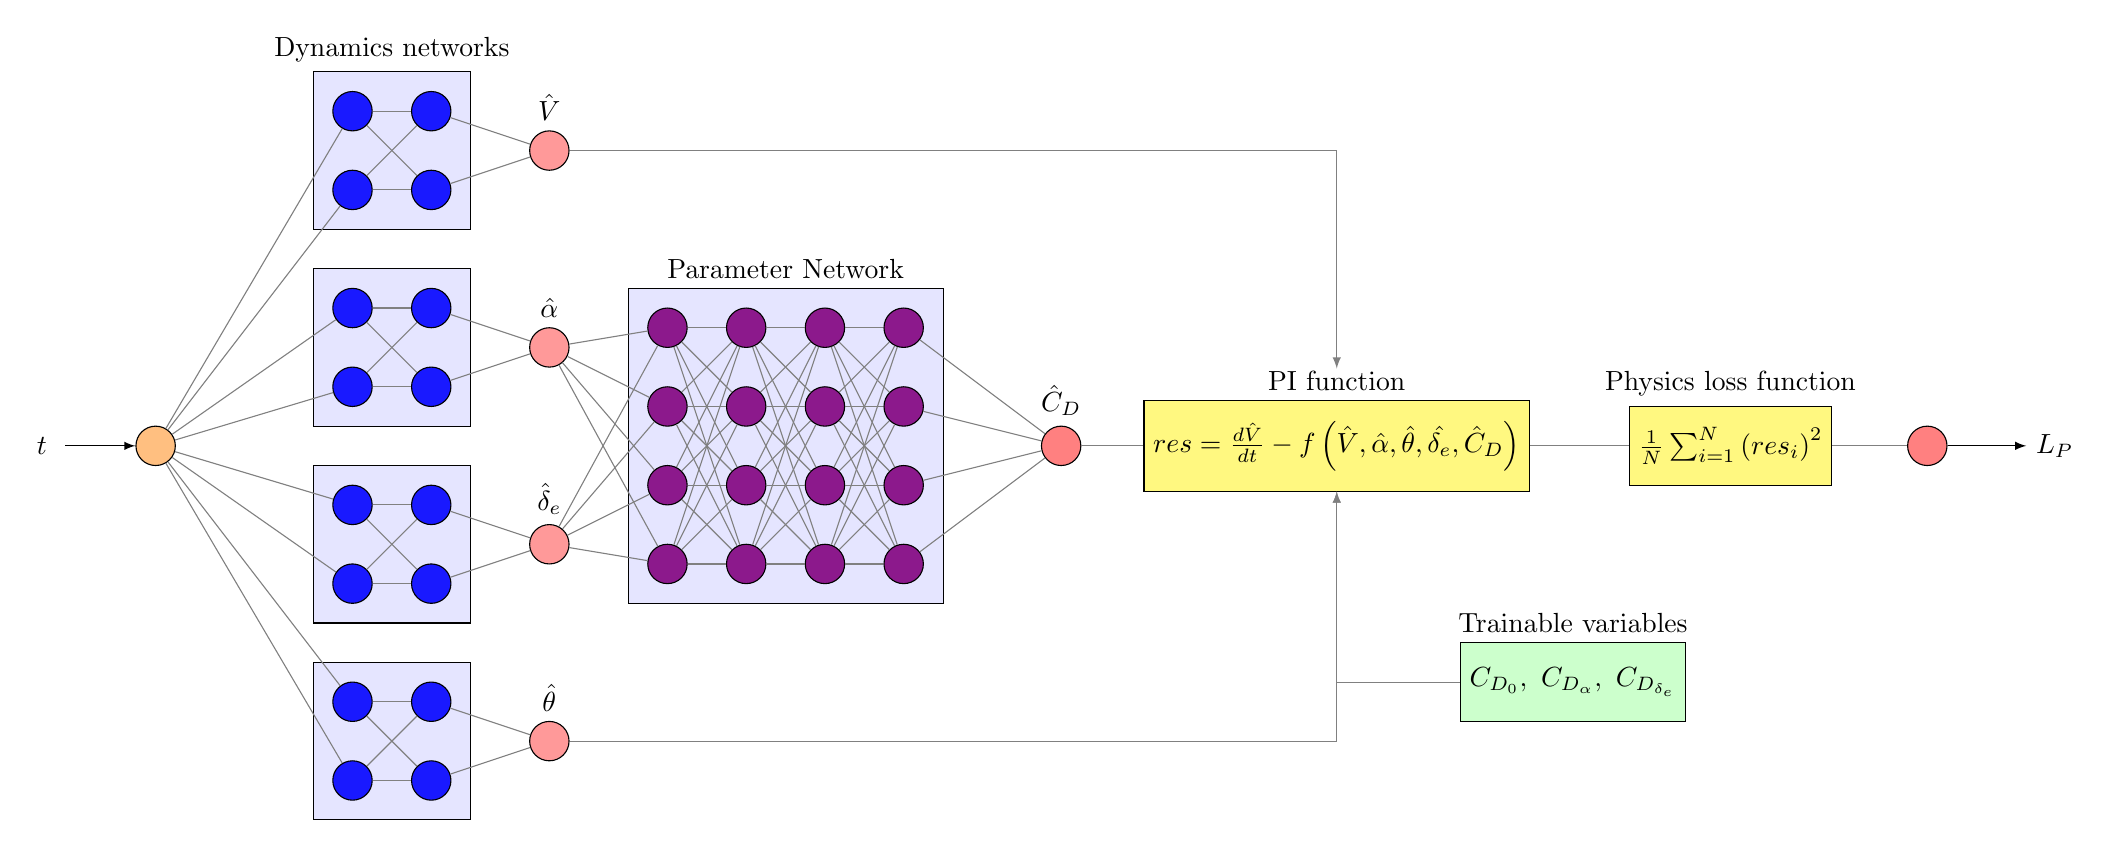
\begin{tikzpicture}

    % drawing boundary box for parameter network
    \node[draw,
    rectangle,
    minimum width = 4cm,
    minimum height = 4cm,
    label = Parameter Network,
    fill = blue!10] (ParameterNetwork) at (\Hoffset,0) {};

    % parameter network nodes
    \foreach \i in {1,...,4}
    {
        \foreach \j in {1,...,4}
        {
            \node[draw,
            circle,
            minimum size = 0.5cm,
            fill=violet!90] (PN_HL-\i-\j) at (-2.5+\j+\Hoffset,2.5-\i){};
        }
    }

    % C_D node
    \node[draw,
    circle,
    minimum size = 0.5cm,
    label = \(\hat{C}_D\),
    fill=red!50] (CD) at (3.5+\Hoffset,0) {};

    % PI function node
    \node[draw,
    rectangle,
    minimum width = 2cm,
    minimum height = 1.15cm,
    label = PI function,
    fill = yellow!50] (PI_function) at (7+\Hoffset,0) {\(res = \frac{d \hat{V}}{dt} - f\left(\hat{V},\hat{\alpha},\hat{\theta},\hat{\delta_e},\hat{C}_D\right)\)};

    % physics loss function
    \node[draw,
    rectangle,
    minimum width = 1cm,
    minimum height = 1cm,
    label = Physics loss function,
    fill = yellow!50] (PI_loss_function) at (12+\Hoffset,0) {\(\frac{1}{N}\sum_{i=1}^N\left(res_i\right)^2\)};

    % physics loss node
    \node[draw,
    circle,
    minimum size = 0.5cm,
    fill=red!50] (LP) at (14.5+\Hoffset,0) {};

    % % backpropagation notation node
    % \node[draw,
    %     rectangle,
    %     minimum width = 1cm,
    %     minimum height = 0.1cm,
    %     fill = teal!30] (BackPropagation) at (8+\Hoffset,-5) {Back Propagation};

    % trainable variables box definition
    \node[draw,
    rectangle,
    minimum width = 1cm,
    minimum height = 1cm,
    label = Trainable variables,
    fill = green!20] (TrainableVariables) at (10+\Hoffset, -3) {\(C_{D_0}, \ C_{D_\alpha}, \ C_{D_{\delta_e}}\)};

    % adding connections to the parameter network part-------------------------
    \foreach \i in {1,...,4}
    {
        \foreach \j in {1,...,4}
        {
            \draw[color=black!50] (PN_HL-\i-1) -- (PN_HL-\j-2);
            \draw[color=black!50] (PN_HL-\i-2) -- (PN_HL-\j-3);
            \draw[color=black!50] (PN_HL-\i-3) -- (PN_HL-\j-4);
        }
        \draw[color=black!50] (PN_HL-\i-4) -- (CD);
    }
    \draw[color=black!50] (CD) -- (PI_function);
    \draw[color=black!50] (PI_function) -- (PI_loss_function);
    \draw[color=black!50] (PI_loss_function) -- (LP);
    \draw[-latex,color=black!50] (TrainableVariables.west) -| (PI_function);
    \draw[-latex] (LP.east) -- ++(1,0) node[right]{\(L_{P}\)};
    % \draw[color=black!50] (LP) |- (BackPropagation.east);
    % \draw[-latex,color=black!50] (BackPropagation) -| (ParameterNetwork.south);

    % adding V network---------------------------------------------------------

    % hidden layer cover
    \node[draw,
    rectangle,
    minimum width = 2 cm,
    minimum height = 2 cm,
    label = Dynamics networks,
    fill=blue!10] (V_HiddenLayerRectangle) at (2.0,0+\VVoffset){};

    % hidden layer neurons
    \foreach \i in {1,...,2}
    {
        \node[draw,
        circle,
        minimum size = 0.5 cm,
        fill=blue!90] (V_HL_CL_1-\i)  at (1.5, \i-1.5+\VVoffset){};
    }

    \foreach \i in {1,...,2}
    {
        \node[draw,
        circle,
        minimum size = 0.5 cm,
        fill=blue!90] (V_HL_CL_2-\i)  at (2.5, \i-1.5+\VVoffset){};
    }

    % output nodes
    \node[draw,
    circle,
    minimum size = 0.5 cm,
    label = \(\hat{V}\),
    fill=red!40] (V_hat) at (4.0,0.0+\VVoffset){};

    % adding alpha network-----------------------------------------------------
    % hidden layer cover
    \node[draw,
    rectangle,
    minimum width = 2 cm,
    minimum height = 2 cm,
    fill=blue!10] (alpha_HiddenLayerRectangle) at (2.0,0+\alphaVoffset){};

    % hidden layer neurons
    \foreach \i in {1,...,2}
    {
        \node[draw,
        circle,
        minimum size = 0.5 cm,
        fill=blue!90] (alpha_HL_CL_1-\i)  at (1.5, \i-1.5+\alphaVoffset){};
    }

    \foreach \i in {1,...,2}
    {
        \node[draw,
        circle,
        minimum size = 0.5 cm,
        fill=blue!90] (alpha_HL_CL_2-\i)  at (2.5, \i-1.5+\alphaVoffset){};
    }

    % output nodes
    \node[draw,
    circle,
    minimum size = 0.5 cm,
    label = \(\hat{\alpha}\),
    fill=red!40] (alpha_hat) at (4.0,0.0+\alphaVoffset){};

    % adding dele network------------------------------------------------------
    % hidden layer cover
    \node[draw,
    rectangle,
    minimum width = 2 cm,
    minimum height = 2 cm,
    fill=blue!10] (dele_HiddenLayerRectangle) at (2.0,0+\deleVoffset){};

    % hidden layer neurons
    \foreach \i in {1,...,2}
    {
        \node[draw,
        circle,
        minimum size = 0.5 cm,
        fill=blue!90] (dele_HL_CL_1-\i)  at (1.5, \i-1.5+\deleVoffset){};
    }

    \foreach \i in {1,...,2}
    {
        \node[draw,
        circle,
        minimum size = 0.5 cm,
        fill=blue!90] (dele_HL_CL_2-\i)  at (2.5, \i-1.5+\deleVoffset){};
    }

    % output nodes
    \node[draw,
    circle,
    minimum size = 0.5 cm,
    label = \(\hat{\delta}_e\),
    fill=red!40] (dele_hat) at (4.0,0.0+\deleVoffset){};

    % adding theta network-----------------------------------------------------
    % hidden layer cover
    \node[draw,
    rectangle,
    minimum width = 2 cm,
    minimum height = 2 cm,
    fill=blue!10] (theta_HiddenLayerRectangle) at (2.0,0+\thetaVoffset){};

    % hidden layer neurons
    \foreach \i in {1,...,2}
    {
        \node[draw,
        circle,
        minimum size = 0.5 cm,
        fill=blue!90] (theta_HL_CL_1-\i)  at (1.5, \i-1.5+\thetaVoffset){};
    }

    \foreach \i in {1,...,2}
    {
        \node[draw,
        circle,
        minimum size = 0.5 cm,
        fill=blue!90] (theta_HL_CL_2-\i)  at (2.5, \i-1.5+\thetaVoffset){};
    }

    % output nodes
    \node[draw,
    circle,
    minimum size = 0.5 cm,
    label = \(\hat{\theta}\),
    fill=red!40] (theta_hat) at (4.0,0.0+\thetaVoffset){};

    % input node---------------------------------------------------------------
    \node[draw,
    circle,
    minimum size = 0.5cm,
    fill = orange!50] (t_input) at (-1,0) {};

    % building connections in the dynamics network-----------------------------
    \foreach \i in {1,...,2}
    {
        % hidden layer connections
        \foreach \j in {1,...,2}
        {
            \draw[color=black!50] (V_HL_CL_1-\j) -- (V_HL_CL_2-\i);
            \draw[color=black!50] (alpha_HL_CL_1-\j) -- (alpha_HL_CL_2-\i);
            \draw[color=black!50] (theta_HL_CL_1-\j) -- (theta_HL_CL_2-\i);
            \draw[color=black!50] (dele_HL_CL_1-\j) -- (dele_HL_CL_2-\i);
        }
        % output node connections
        \draw[color=black!50] (V_HL_CL_2-\i) -- (V_hat);
        \draw[color=black!50] (alpha_HL_CL_2-\i) -- (alpha_hat);
        \draw[color=black!50] (theta_HL_CL_2-\i) -- (theta_hat);
        \draw[color=black!50] (dele_HL_CL_2-\i) -- (dele_hat);
        % input node connections
        \draw[color=black!50] (V_HL_CL_1-\i) -- (t_input);
        \draw[color=black!50] (alpha_HL_CL_1-\i) -- (t_input);
        \draw[color=black!50] (theta_HL_CL_1-\i) -- (t_input);
        \draw[color=black!50] (dele_HL_CL_1-\i) -- (t_input);
    }
    % state output to parameter network connections
    \foreach \i in {1,...,4}
    {
        \draw[color=black!50] (PN_HL-\i-1) -- (alpha_hat);
        \draw[color=black!50] (PN_HL-\i-1) -- (dele_hat);
    }
    % V to PI function connection
    \draw[-latex,color=black!50, shorten >= 4mm] (V_hat) -| (PI_function.north);
    % theta to PI function connection
    % \draw[-{Arc Barb[harpoon,reversed]},color = black!50] (theta_hat) -- (7,-3.75);
    % \draw[{Arc Barb[harpoon,reversed,right]}-,color = black!50]  (7,-3.75) -| (PI_function.south);
    \draw[-latex,color=black!50] (theta_hat) -| (PI_function.south);

    % adding input notation
    \draw[latex-, shorten >=1mm] (t_input.west) -- ++(-1.0,00) node[left]{\(t\)};

\end{tikzpicture}

\end{document}
